\documentclass[12pt,xcolor=table,aspectratio=169]{beamer}
\usetheme{Frankfurt}
\usecolortheme{rose}
\usepackage{amsthm}
\usepackage{amsmath}
\usepackage{bbm}
\usepackage{amsfonts}
\usepackage{amssymb}
\usepackage{graphicx}
\usepackage{hyperref}
\usepackage[flushleft]{threeparttable}
\usepackage{tabularx}
\usepackage{booktabs}
\usepackage{siunitx}
\usepackage{tikz}
\usetikzlibrary{decorations.pathreplacing,angles,quotes}
%\usepackage{enumitem}% http://ctan.org/pkg/enumitem

%set up course and number

\newcommand{\ClassName}{TBD}
\newcommand{\ClassNumber}{TBD}
\newcommand{\Topic}{TBD}

% Some optional colors. Change or add as you see fit.
%---------------------------------------------------
 \definecolor{ualbertagreen}{HTML}{007C41}
\definecolor{ualbertagold}{HTML}{FFDB05}

\definecolor{calloutgrey}{HTML}{D9D9D9}


%set fonts
\setbeamerfont{subtitle}{size=\large,shape=\scshape,series=\bfseries}
\setbeamerfont{title}{size=\Large,shape=\scshape,series=\bfseries}
\setbeamerfont{author}{size=\large}
\setbeamerfont{date}{size=\large}
\setbeamerfont{caption}{size=\scriptsize}


% Some optional color adjustments to Beamer. Change as you see fit.
%------------------------------------------------------------------
\setbeamercolor{frametitle}{fg=ualbertagreen,bg=white}
\setbeamercolor{title}{fg=ualbertagreen,bg=white}
\setbeamercolor{author}{fg=ualbertagreen,bg=white}
\setbeamercolor{date}{fg=ualbertagreen,bg=white}
\setbeamercolor{local structure}{fg=ualbertagreen}
\setbeamercolor{section in toc}{fg=ualbertagreen,bg=white}
% \setbeamercolor{subsection in toc}{fg=ualbertagreen,bg=white}
\setbeamercolor{footline}{fg=ualbertagreen!50, bg=white}

% definition boxes
\setbeamercolor{block title}{bg=ualbertagreen,fg=white}
\setbeamercolor{block body}{parent=normal text,use=block title,bg=calloutgrey}
%\setbeamercolor{block body}{parent=normal text,use=block title,bg=block title.bg!30!bg}


\setbeamercolor{upper separation line head}{bg=ualbertagreen}
\setbeamercolor{lower separation line head}{bg=ualbertagold}
\setbeamercolor{middle separation line head}{bg=ualbertagold}
\setbeamercolor{frametitle}{fg=ualbertagreen,bg=white}



\setbeamercolor{section in head/foot}{bg=white,fg=ualbertagreen}
\setbeamercolor{author in head/foot}{bg=white,fg=ualbertagreen}
\setbeamercolor{date in head/foot}{bg=white,,fg=ualbertagreen}
\setbeamercolor{title in head/foot}{bg=white,fg=ualbertagreen}

\setbeamercolor{headline}{bg=white,fg=ualbertagreen}




\setbeamercolor*{middle separation line head}{bg=ualbertagreen}
\setbeamercolor*{alerted text}{fg=ualbertagreen}
\setbeamercolor*{example text}{fg=black}
\setbeamercolor*{structure}{fg=black}


\let\Tiny=\tiny



\logo{
   %\ifnum\insertpagenumber>1
   \tikz [remember picture,overlay]
    \node[yshift=.3cm,xshift=1.5cm] at (current page.south west)
        %or: (current page.center)
        {
\includegraphics[width=1in]{../images/UA-ASB-COLOUR.png}};
    %\fi
%
\includegraphics[height=0.8cm]{../images/UA-ASB-COLOUR.png}\vspace{220pt}
}


\setbeamertemplate{title page}{%
  \vbox{}
    \vspace{.5cm}% NEW
  \begingroup
    \centering
    \begin{beamercolorbox}[sep=8pt,center]{title}
      \usebeamerfont{title}\ClassNumber: \ClassName\par%
      \usebeamerfont{title}\inserttitle\par%
     \ifx\insertsubtitle\@empty%
      \else%
        \vskip0.05em%
        {\usebeamerfont{subtitle}\usebeamercolor[fg]{subtitle}\insertsubtitle\par}%
      \fi%
    \end{beamercolorbox}%
    \begin{beamercolorbox}[sep=8pt,center]{author}
      \usebeamerfont{author}\insertauthor
    \end{beamercolorbox}
    \begin{beamercolorbox}[sep=8pt,center]{institute}
      \usebeamerfont{institute}\insertinstitute
    \end{beamercolorbox}

    \vspace{0.5cm}% NEW
    \begin{beamercolorbox}[sep=8pt,center]{date}
      \usebeamerfont{date}\insertdate
    \end{beamercolorbox}\vskip0.05em

      \endgroup
  %\vfill
}


\setbeamertemplate{frametitle}{%
    \insertframetitle\par\vskip-10pt
}



\renewcommand{\ClassName}{Business Economics, Organization and Management}
\renewcommand{\ClassNumber}{BUEC 311}

\setbeamertemplate{headline}{%
\leavevmode%
 \hbox{%
    \begin{beamercolorbox}[wd=\paperwidth,ht=5ex,dp=0ex]{white}%
    \usebeamerfont{headline}\hskip6pt\ClassNumber: \inserttitle\par%
    \insertsectionnavigationhorizontal{\paperwidth}{}{\hskip0pt plus1filll}
    \end{beamercolorbox}%
  }
}

\defbeamertemplate*{footline}{my footline}{%
    \ifnum\insertpagenumber=1
        \Tiny{%
            \hfill%
		\vspace*{1pt}%
            %\insertframenumber/\inserttotalframenumber \hspace*{0.1cm}%
            \newline%
            \color{ualbertagold}{\rule{\paperwidth}{0.4mm}}\newline%
            \color{ualbertagold}{\rule{\paperwidth}{.4mm}}%
        }
  \else%
        \Tiny{%
            \hspace{.66\paperwidth}
            %\vspace{25pt}
            \insertframenumber/\inserttotalframenumber
            \newline%
            \color{ualbertagold}{\rule{\paperwidth}{0.4mm}}\newline%
            \color{ualbertagold}{\rule{\paperwidth}{.4mm}}%
        }%
    \fi%
}


\newenvironment{itemize*}%
  {\begin{itemize}%
    \setlength{\itemsep}{0pt}%
    \setlength{\parskip}{0pt}}%
  {\end{itemize}}


\title{Government Intervention
}

\date{Fall 2020}

\begin{document}

\frame{
	\titlepage
}
\section{Overview}

\frame{
	\frametitle{Outline}
	\begin{enumerate}
	\item Market Failure and Government Policy
	\item[]
	\item Regulation of Imperfectly Competitive Markets
	\item[]
	\item Antitrust Law and Competition Policy
	\item[]
	\item Externalities
	\item[]
	\item Open-Access, Club, and Public Goods
	\item[]
	\item Intellectual Property
	\end{enumerate}
}

\frame{
	\frametitle{Government Intervention}
	\begin{itemize}
	\item Now we will examine how/why governments intervene in the market.
	\item[]
	\item Two main motives for government response:
		\begin{enumerate}
		\item \underline{Market failures} caused by non-competitive market structures.
			\begin{itemize}
			\item Response may be \underline{regulation}, \underline{antitrust}, or \underline{competition policy}.
			\end{itemize}
		\item \underline{Market failures} caused by externalities.
			\begin{itemize}
			\item A market failure that arises due to incomplete property rights.
			\end{itemize}
		\end{enumerate}
	\item[]
	\item \underline{Idea}: Government is trying to eliminate deadweight loss created by market failures.
	\end{itemize}
}

\section{Market Failure}

\frame{
	\frametitle{Outline}
	\begin{enumerate}
	\item \alert{Market Failure and Government Policy}
	\item[]
	\item Regulation of Imperfectly Competitive Markets
	\item[]
	\item Antitrust Law and Competition Policy
	\item[]
	\item Externalities
	\item[]
	\item Open-Access, Club, and Public Goods
	\item[]
	\item Intellectual Property
	\end{enumerate}
}

\frame{
	\frametitle{Market Failure and Government Policy}
	\begin{itemize}
	\item \underline{Recall}: Perfectly competitive markets achieve economic efficiency and maximize total surplus.
	\item[]
	\item However, in practice, most markets exhibit market failures.
		\begin{itemize}
		\item Implication: potential substantial welfare losses.
		\end{itemize}
	\item[]
	\item Deadweight loss created by market failures creates a rationale for government intervention:
		\begin{itemize}
		\item Try to reduce/eliminate market failure.
		\end{itemize}
	\item[]
	\item But is government intervention desirable.
	\end{itemize}
}

\frame{
	\frametitle{Market Failure and Government Policy}
	\begin{itemize}
	\item Economists evaluate the desirability of government policy in two ways:
		\begin{enumerate}
		\item \underline{Pareto principle}: A policy is desirable if it yields a \underline{Pareto improvement}.
			\begin{itemize}
			\item A Pareto improvement is any reallocation of goods or productive inputs that helps at least one person, \textit{without harming anyone else}.
			\end{itemize}
		\item \underline{Cost-Benefit principle}: A policy is desirable if its benefits exceed the costs.
			\begin{itemize}
			\item Any policy that increases total surplus is desirable even if some will be harmed.
			\end{itemize}
		\end{enumerate}
	\item[]
	\item Two points to note:
		\begin{enumerate}
		\item Any policy that generates a Pareto improvement satisfies the cost-benefit principle, but the converse is not necessarily true.
		\item In practice, policies that have large net benefits and small distributional effects tend to have broad support. Policies with small net benefits and/or large distributional effects are likely to be contentious.
		\end{enumerate}
	\end{itemize}
}


\section{Competition}

\frame{
	\frametitle{Outline}
	\begin{enumerate}
	\item Market Failure and Government Policy
	\item[]
	\item \alert{Regulation of Imperfectly Competitive Markets}
	\item[]
	\item Antitrust Law and Competition Policy
	\item[]
	\item Externalities
	\item[]
	\item Open-Access, Club, and Public Goods
	\item[]
	\item Intellectual Property
	\end{enumerate}
}

\frame{
	\frametitle{Eliminating Market Failure Due to Imperfect Competition}
	\begin{itemize}
	\item Three approaches governments can use to address the market failure created by imperfectly competitive pricing:
		\begin{enumerate}
		\item In the case of a monopoly: Own the monopolist and set relatively low prices.
			\begin{itemize}
			\item Ex: Government ownership of electric power/water utilities.
			\end{itemize}
		\item[]
		\item Regulate firms to prevent them from setting excessively high prices.
		\item[]
		\item Change market structure using antitrust or competition policy.
		\end{enumerate}
	\end{itemize}
}

\frame{
	\frametitle{Regulation of Imperfectly Competitive Markets}
	\begin{itemize}
	\item Most common approach to correcting market failure arising from imperfect competition: Price Ceiling or \underline{Price Cap}.
		\begin{itemize}
		\item Ex: Price caps are used to regulate telecommunications monopolies in 33 U.S. states, and Australia, Canada, Denmark, France, Germany, Mexico and the U.K.
		\end{itemize}
	\item[]
	\item \underline{Idea}: Government can eliminate deadweight loss by imposing a price cap equal to the price that would prevail in a competitive market.
	\end{itemize}
}

\frame{
	\frametitle{Regulation of Imperfectly Competitive Markets}
	\begin{figure}
	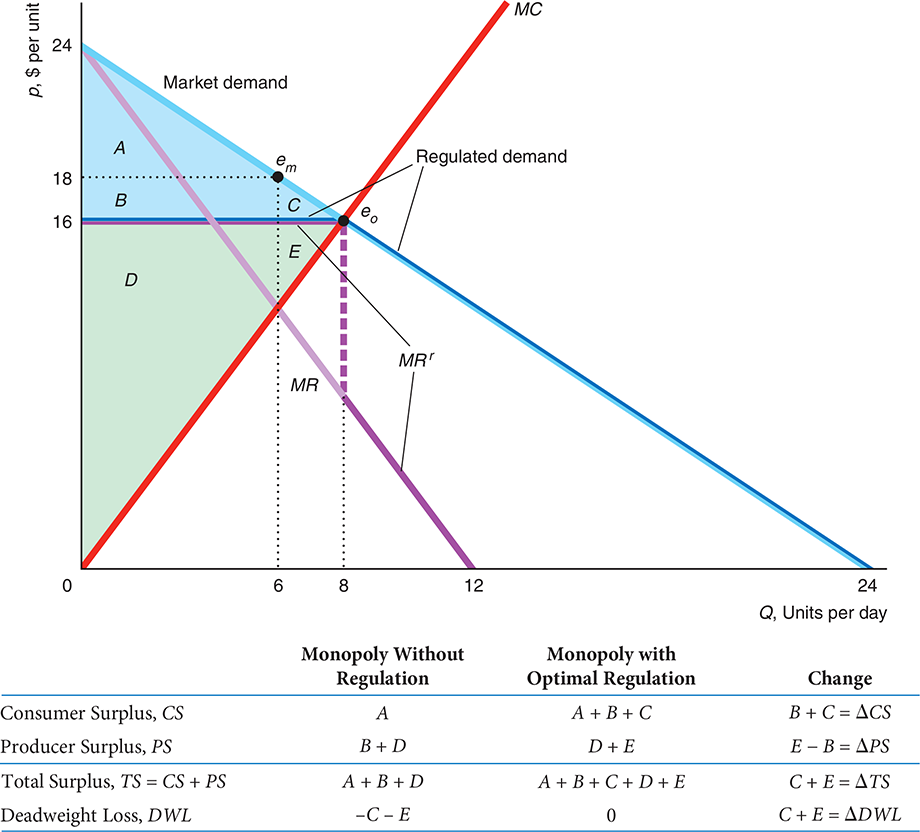
\includegraphics[scale=0.25]{../images/intervention/price_cap.png}
	\end{figure}
}

\frame{
	\frametitle{Regulation of Imperfectly Competitive Markets}
	\begin{itemize}
	\item Would a government always be able to eliminate deadweight loss using a price cap?
	\end{itemize}
}

\frame{
	\frametitle{Regulation of Imperfectly Competitive Markets}
	\begin{itemize}
	\item Regulation can be sub-optimal for several reasons:
		\begin{enumerate}
		\item Poor information about demand and/or costs.
			\begin{itemize}
			\item Limited information may lead to a price cap set above or below the efficient level.
			\end{itemize}
		\item[]
		\item Inability to subsidize.
			\begin{itemize}
			\item If a monopolist exhibits economies of scale, it may require a subsidy to produce the efficient level, which may not be politically viable.
			\end{itemize}
		\item[]
		\item Regulatory capture.
			\begin{itemize}
			\item Many firms engage in \underline{rent seeking} (they devote effort and expenditures to gain a ``rent'' or profit from government actions) to \underline{capture} the regulator.
			\item A captured regulator will put industry interests ahead of the public interest.
			\end{itemize}
		\end{enumerate}
	\end{itemize}
}

\frame{
	\frametitle{Regulation of Imperfectly Competitive Markets}
	\begin{itemize}
	\item Issues of information/subsidization/capture aside, it is important to recognize that regulating markets where $p>MC$ may still not be socially desirable because enacting regulation is costly.
		\begin{itemize}
		\item Costs include gathering information, mistakes, regulatory capture/rent seeking.
		\end{itemize}
	\item[]
	\item Governments should only regulate when doing so passes a cost-benefit test.
		\begin{itemize}
		\item Typically this will be when market failures are large; in this case, the benefits from reducing a market failure will most likely exceed the costs.
		\end{itemize}
	\end{itemize}
}

\section{Anti-Trust Law}

\frame{
	\frametitle{Outline}
	\begin{enumerate}
	\item Government Intervention
	\item[]
	\item Market Failure and Government Policy
	\item[]
	\item Regulation of Imperfectly Competitive Markets
	\item[]
	\item \alert{Antitrust Law and Competition Policy}
	\item[]
	\item Externalities
	\item[]
	\item Open-Access, Club, and Public Goods
	\item[]
	\item Intellectual Property
	\end{enumerate}
}

\frame{
	\frametitle{Antitrust Law and Competition Policy}
	\begin{itemize}
	\item Rather than directly regulating firms that set high prices, governments can instead enact laws that forbid firms from forming cartels and collectively setting high prices.
		\begin{itemize}
		\item These laws are referred to as \textit{antitrust laws} (U.S.) or \textit{competition policies} (Canada).
			\begin{itemize}
			\item Canada's first antitrust law: 1889.
			\item America's first antitrust law: 1890.
			\end{itemize}
		\item[]
		\item Laws are administered by government bodies.
			\begin{itemize}
			\item Canada: Competition Bureau
			\item U.S.: Department of Justice (DOJ), and the Federal Trade Commission (FTC)
			\end{itemize}
		\item[]
		\item In both the U.S. and Canada, price fixing is \textit{per-se} illegal.
			\begin{itemize}
			\item It is strictly against the law, there are no possible mitigating justifications.
			\item Subject to criminal and civil punishments.
			\end{itemize}
		\end{itemize}
	\end{itemize}
}

\frame{
	\frametitle{Antitrust Law and Competition Policy}
	\begin{itemize}
	\item Antitrust laws also govern mergers, predatory actions, and vertical relationships.
		\begin{itemize}
		\item \underline{Mergers}: Most antitrust and competition law restricts the ability of firms to merge if the net effect is to harm society.
			\begin{itemize}
			\item Key question: Do benefits of increased efficiency outweigh costs of reduced competition?
			\end{itemize}
		\item[]
		\item \underline{Predatory Actions}: Most antitrust laws prevent \underline{predatory pricing}.
			\begin{itemize}
			\item Prevents firms from setting $p$ below $MC$ or $AC$ to drive rivals out of business and then raising their price.
			\item This can be difficult for a regulator to demonstrate; it requires that rivals must not be able to re-enter when the price is increased.
			\end{itemize}
		\end{itemize}
	\end{itemize}
}

\frame{
	\frametitle{Antitrust Law and Competition Policy}
	\begin{itemize}
	\item \underline{Vertical relationships} refer to vertical interactions between a firm and its customers or suppliers.
	\item[]
	\item Competition authorities focus on four key vertical actions:
		\begin{enumerate}
		\item \underline{Resale price maintenance} (RPM): Occurs when a manufacturer \textit{requires} that retailers who sell its product charge no lower than a specified price.
			\begin{itemize}
			\item Usually legal if a manufacturer acts unilaterally.
			\end{itemize}
		\item \underline{Refusal to deal}: Occurs when dominant integrated firm operating upstream and downstream refuses to sell to downstream competitors.
			\begin{itemize}
			\item Needs a sound basis for refusal; motive cannot be to harm competitors.
			\end{itemize}
		\item \underline{Exclusive dealing}: Occurs when a firm sells its product only to customers who agree to buy from that firm and not its rivals.
			\begin{itemize}
			\item Only problematic if it reduces market competition.
			\end{itemize}
		\item \underline{Price discrimination}: Legal unless it harms competition.
		\end{enumerate}
	\end{itemize}
}

\section{Externalities}

\frame{
	\frametitle{Outline}
	\begin{enumerate}
	\item Market Failure and Government Policy
	\item[]
	\item Regulation of Imperfectly Competitive Markets
	\item[]
	\item Antitrust Law and Competition Policy
	\item[]
	\item \alert{Externalities}
	\item[]
	\item Open-Access, Club, and Public Goods
	\item[]
	\item Intellectual Property
	\end{enumerate}
}

\frame{
	\frametitle{5. Externalities}
	\begin{itemize}
	\item An \underline{externality} occurs when a person's well being, or a firm's production capability is \underline{directly} affected by the actions of other consumers or firms rather than \underline{indirectly} through changes in \underline{prices}.
		\begin{itemize}
		\item Effect is external because it occurs \textit{outside} of the market and, hence, has not price.
		\end{itemize}
	\item Externalities can be negative or positive.
		\begin{itemize}
		\item A negative externality harms others:
			\begin{itemize}
			\item Ex. A chemical plant that dumps waste into a lake, reducing the profits of a firm that rents boats.
			\end{itemize}
		\item A positive externality helps others:
			\begin{itemize}
			\item Ex. A homeowner that invests a lot in landscaping on his/her property increases the value of neighbours' homes too.
			\end{itemize}
		\end{itemize}
	\end{itemize}
}

\frame{
	\frametitle{Externalities}
	\begin{itemize}
	\item When activities create externalities, the competitive market outcome will be inefficient.
	\item[]
	\item As an example, consider a competitive market in which firms produce paper.
		\begin{itemize}
		\item Paper production creates pollution emission as a byproduct.
		\item Pollution harms people who live near paper mills.
		\item Assume, to start, that the paper mills do not have to pay for the harm that their pollution emissions cause.
		\end{itemize}
	\end{itemize}
}

\frame{
	\frametitle{Externalities}
	\begin{itemize}
	\item Because firms do not pay for the harm that their pollution causes, they only consider \underline{direct costs} associated with production (labor, capital, energy, wood pulp, etc) when choosing how much to produce; the \underline{indirect costs} created by the harm from the externality are ignored.
	\item[]
	\item The \underline{social cost} associated with paper production is the sum of direct and indirect costs.
		\begin{itemize}
		\item It is the total cost to society.
		\end{itemize}
	\item[]
	\item If the firms do not pay for the harm that their pollution causes, the competitive market produces excessive pollution because \textit{each firm's private, direct cost is less than the social cost}.
	\end{itemize}
}

\frame{
	\frametitle{Externalities}
	\begin{figure}
	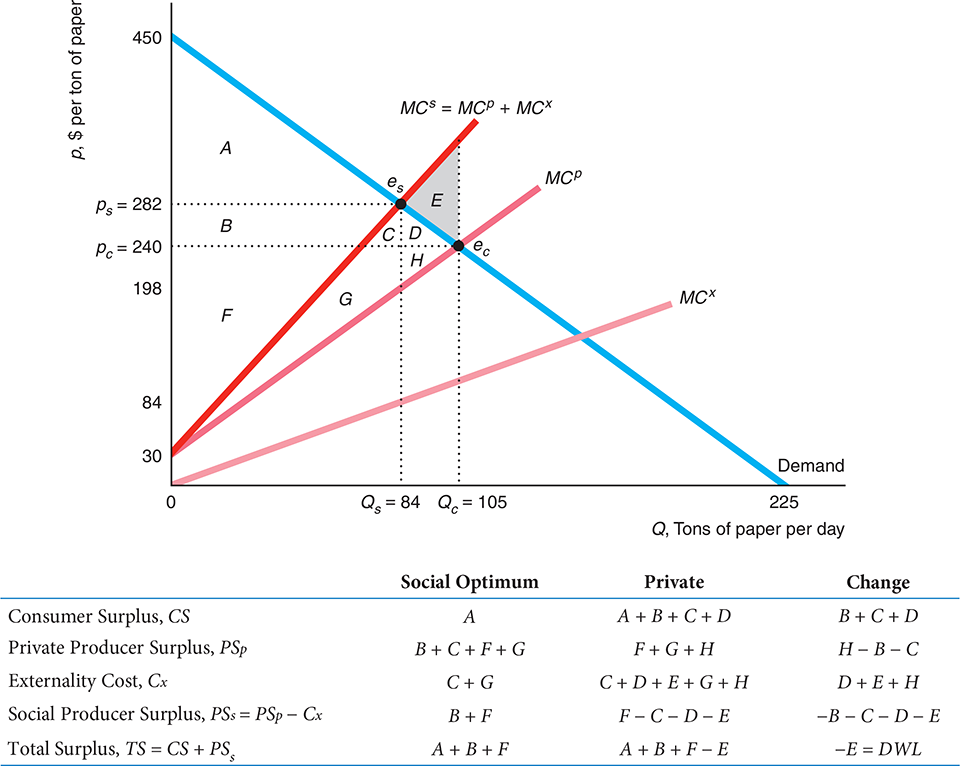
\includegraphics[scale=0.25]{../images/intervention/social_cost.png}
	\end{figure}
}

\frame{
	\frametitle{Externalities}
	\begin{itemize}
	\item If the government has sufficient knowledge about the harm caused by pollution, the demand curve, costs, and production technologies, it can force a competitive market to produce the socially optimal level of output.
	\item[]
	\item The government can control pollution directly by setting \underline{emission standards}, or by taxing pollution with an \underline{emissions fee} or an \underline{effluent change}.
		\begin{itemize}
		\item It can also control pollution indirectly by limiting outputs are inputs.
		\end{itemize}
	\end{itemize}
}

\frame{
	\frametitle{Externalities}
	\begin{figure}
	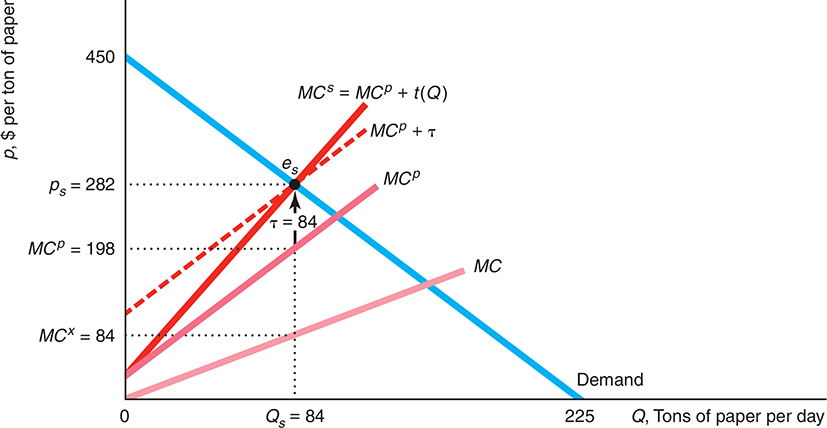
\includegraphics[scale=0.45]{../images/intervention/tax.png}
	\end{figure}
}	

\frame{
	\frametitle{Pollution and Property Rights}
	\begin{itemize}
	\item Another approach to solving the externality problem is for the government or courts to clearly assign \underline{property rights} over pollution.
		\begin{itemize}
		\item Idea: Give polluter right to pollute, or affected party the right to be free from pollution.
			\begin{itemize}
			\item If clear property rights can be established, pollution can be priced, and the externality problem can be reduced or eliminated.
			\item \underline{Coase theorem:} A polluter and its victim can achieve the optimal level of pollution if property rights are clearly defined and the parties can bargain effectively.
			\end{itemize}
		\end{itemize}
	\item[]
	\item As an example of how property rights can solve the externality problem, consider Secret Garden Tea House \& Fixit Car-Body Shop.
		\begin{itemize}
		\item Fixit create loud noises fixing cars that reduces Secret Garden's profits.
		\end{itemize}
	\end{itemize}
}

\frame{
	\frametitle{Pollution and Property Rights}
	\begin{figure}
	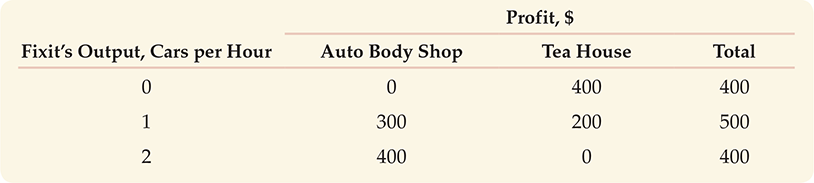
\includegraphics[scale=0.5]{../images/intervention/coase.png}
	\caption{Payoffs to Secret Garden \& Fixit}
	\end{figure}
}

\frame{
	\frametitle{Pollution and Property Rights}
	\begin{itemize}
	\item Initially, suppose that there are not property rights over noise. In this case Fixit will not negotiate with Secret Garden; it has no incentive to do so.
		\begin{itemize}
		\item Outcome: Fixit works on two cars per hour and makes \$400. The excessive noise drives Secret Garden out of business. Joint profit: \$400.
		\end{itemize}
	\item Now, instead suppose that Secret Garden is given the \underline{right to silence}.
		\begin{itemize}
		\item Secret Garden now has property rights; it can force Fixit to shut down.
		\item However, shutting Fixit down is not necessarily the best option:
			\begin{itemize}
			\item If Fixit shuts down, Secret Garden makes \$400. Joint profit: \$400.
			\item If Fixit produces one car, it earns \$300, and Secret Garden makes \$200. Join profit: \$500.
			\item Firms should reach an agreement where Fixit pays Secret Garden between \$200 and \$300 for the right to work on one car.
			\end{itemize}
		\end{itemize}
	\item If Fixit gets the right to noise, a similar beneficial outcome occurs.
	\end{itemize}
}

\frame{
	\frametitle{Coase Theorem}
	\begin{itemize}
	\item Lessons from the Coase Theorem:
		\begin{enumerate}
		\item If property rights are not clear, the agent that produces negative externality produces too much and joint profit is not maximized.
		\item Assigning property rights maximizes joint profit, regardless of how property rights are assigned.
		\item Who gets property rights affects the \textit{distribution} of joint profit.
		\end{enumerate}
	\item[]
	\item Limitations of the Coase Theorem:
		\begin{itemize}
		\item Bargaining may not be possible because of high transaction costs.
		\item If parties lack information about the costs or benefits of reducing negative externality, bargaining is not possible.
		\end{itemize}
	\end{itemize}
}

\frame{
	\frametitle{Outline}
	\begin{enumerate}
	\item Market Failure and Government Policy
	\item[]
	\item Regulation of Imperfectly Competitive Markets
	\item[]
	\item Antitrust Law and Competition Policy
	\item[]
	\item Externalities
	\item[]
	\item \alert{Open-Access, Club, and Public Goods}
	\item[]
	\item Intellectual Property
	\end{enumerate}
}

\frame{
	\frametitle{Open-Access, Club, And Public Goods}
	\begin{itemize}
	\item The characteristics of goods and services can also create motives for government intervention.
	\item[]
	\item Goods and services differ in their \underline{rivalry} and \underline{excludability}.
		\begin{itemize}
		\item Rivalry:
			\begin{itemize}
			\item A good exhibits rivalry if its consumption by one individual means that no one else can consume it (ex: an orange).
			\item A good is non-rival if its consumption by one individual means that anyone else can consume it (ex: clean air).
			\end{itemize}
		\item Excludability:
			\begin{itemize}
			\item A good is excludable if the owner of a good can prevent others from consuming it.
			\item A good is non-excludable if the owner of the good cannot prevent others from consuming it.
			\end{itemize}
		\end{itemize}
	\end{itemize}
}

\frame{
	\frametitle{Open-Access, Club, And Public Goods}
	\begin{figure}
	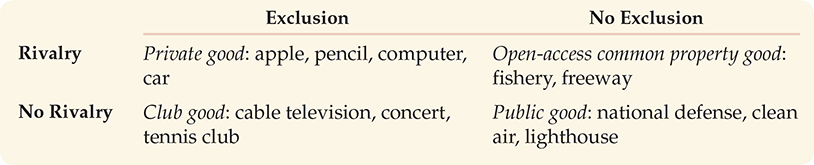
\includegraphics[scale=0.5]{../images/intervention/goods.png}
	\caption{Classification of Goods and Services}
	\end{figure}
}

\frame{
	\frametitle{Open-Access}
	\begin{itemize}
	\item Open-access common property is non-exclusive, but rival.
		\begin{itemize}
		\item Typical of many natural resources.
			\begin{itemize}
			\item Ex: An open-access fishery: Anyone can fish, but fish is rival.
			\end{itemize}
		\item[]
		\item Open access means that the resource is overexploited.
			\begin{itemize}
			\item Ex: Each fisher wants to catch a given fish to gain property fights to that fish; they ignore the \underline{externality cost} from reduced current and future fish populations. This leads to overfishing.
			\item Similar problems arise with water, oil and natural gas, public freeways.
			\end{itemize}
		\item[]
		\item Government regulation can solve the overexploitation problem by restricting access to the commons.
			\begin{itemize}
			\item Typical approaches: First-come, first-served; charging entry fee/tax.
			\item Alternative approach: Assign property rights to create common property.
			\end{itemize}
		\end{itemize}
	\end{itemize}
}

\frame{
	\frametitle{Club Goods}
	\begin{itemize}
	\item Club goods are non-rival, but are subject to exclusion.
		\begin{itemize}
		\item Common example: Golf or Country clubs.
			\begin{itemize}
			\item Clubs exclude people who do not pay membership fees, but services provided (swimming or golfing), are non-rival until full capacity is reached.
			\item Problem: The marginal cost for the club of accepting an additional member is close to zero, but clubs charge more than that. This is a market failure, creates a deadweight loss.
			\end{itemize}
		\item Another example: Cable TV/Streaming Services
			\begin{itemize}
			\item Need to pay to access (exclusion), but one individual?s use does not affect another (non-rival).
			\item Market failure from price above marginal cost.
			\end{itemize}
		\end{itemize}
	\item[]
	\item Government intervention to reduce deadweight loss from club goods is rare.
		\begin{itemize}
		\item A firm may shut down if it is forced to sell at low (zero) marginal cost, creating larger deadweight loss.
		\end{itemize}
	\end{itemize}
}

\frame{
	\frametitle{Public Goods}
	\begin{itemize}
	\item Public goods are non-rival and nonexclusive.
		\begin{itemize}
		\item Ex: Clean air, security, national defence.
			\begin{itemize}
			\item If a firm reduces its pollution (cleans the air), it provides a non-priced benefit to its neighbours; a positive externality.
			\end{itemize}
		\end{itemize}
	\item[]
	\item Public goods are typically undersupplied because of property rights are not clearly defined.
		\begin{itemize}
		\item Issue: Because good is non-exclusive, individuals can benefit from the actions of others without paying.
			\begin{itemize}
			\item People benefit from cleaning efforts of a firm without paying, so it is difficult for a firm to profitably provide clean air.
			\end{itemize}
		\item Consequence: Public goods are under-supplied by markets.
		\end{itemize}
	\item[]
	\item Governments can eliminate the free rider problem by providing goods directly.
		\begin{itemize}
		\item Other solutions require governmental or collective actions such as social pressure, mergers, privatization or mandates.
		\end{itemize}
	\end{itemize}
}


\section{Intellectual Property}

\frame{
	\frametitle{Outline}
	\begin{enumerate}
	\item Market Failure and Government Policy
	\item[]
	\item Regulation of Imperfectly Competitive Markets
	\item[]
	\item Antitrust Law and Competition Policy
	\item[]
	\item Externalities
	\item[]
	\item Open-Access, Club, and Public Goods
	\item[]
	\item \alert{Intellectual Property}
	\end{enumerate}
}

\frame{
	\frametitle{Intellectual Property}
	\begin{itemize}
	\item Intellectual property: property rights over knowledge.
		\begin{itemize}
		\item Issue: knowledge is a public good. It is non-rival and non-exclusive.
			\begin{itemize}
			\item Creates a free rider problem; firms can benefit from discoveries of rivals without paying the research cost.
			\item Such free riding limits the incentive to innovate.
			\end{itemize}
		\end{itemize}
	\item[]
	\item Typical approach to correct free rider problem: \underline{patents} and \underline{copyrights}.
	\item[]
	\item But intellectual property rights create an alternative problem: monopoly power.
		\begin{itemize}
		\item To avoid this governments may fund research with the goal of making findings public or open source.
		\item Another alternative: using innovation prizes.
		\end{itemize}
	\end{itemize}
}

\frame{
	\frametitle{Takeaways}
	\begin{enumerate}
	\item Governments may intervene in markets to correct market failures arising from non-competitive market structures or externalities.
		\begin{itemize}
		\item Characteristics of goods can also create a motive for government involvement in market.
		\end{itemize}
	\item[]
	\item Optimal intervention requires lots of information about the market.
	\item[]
	\item Intervention should only occur if the benefits exceed the costs.
	\end{enumerate}
}

\end{document}

